\documentclass[12pt,titlepage]{article}
\usepackage[dvipsnames,rgb,dvips,table]{xcolor}
\usepackage{graphicx}
\graphicspath{Figures/}
\usepackage{psfrag}
\usepackage{dcolumn}
\usepackage{bm}
\usepackage{amsmath}
\usepackage{amssymb}
\usepackage[rflt]{floatflt}
\usepackage{latexsym}
%\usepackage{float}
\usepackage{bm}
\usepackage{subcaption}
\usepackage{booktabs}
\usepackage{floatrow}
\floatsetup[table]{font=footnotesize}
\usepackage[hidelinks]{hyperref}

%\captionsetup{width=1.1\textwidth}

\usepackage{geometry}
 \geometry{
 left=20mm,
 right=20mm,
 top=25mm,
 bottom=20mm,
 }


\pagestyle{myheadings}
\markright{{\small Jacopo Credi  (910216-T396) \,}}
\DeclareMathOperator\erf{erf}
\author{Jacopo Credi \\(910216-T396) \\ \vspace*{2cm} }
\title{{\Large \textsc{Chalmers University of Technology}} \\ \bigskip FFR105 - Stochastic Optimization Algorithms\\ \bigskip Problem set 2 \\ \vspace*{2cm}}

\usepackage{listings}
\usepackage{color} %red, green, blue, yellow, cyan, magenta, black, white
\definecolor{mygreen}{RGB}{28,172,0} % color values Red, Green, Blue
\definecolor{mylilas}{RGB}{170,55,241}
% Settings for writing Matlab code
\lstset{language=Matlab,%
	basicstyle=\small\ttfamily,
    %basicstyle=\color{red},
    breaklines=true,%
    morekeywords={matlab2tikz},
    keywordstyle=\color{blue},%
    morekeywords=[2]{1}, keywordstyle=[2]{\color{black}},
    identifierstyle=\color{black},%
    stringstyle=\color{mylilas},
    commentstyle=\color{mygreen},%
    showstringspaces=false,%without this there will be a symbol in the places where there is a space
    numbers=left,%
    numberstyle={\tiny \color{black}},% size of the numbers
    numbersep=9pt, % this defines how far the numbers are from the text
    %emph=[1]{for,end,break},emphstyle=[1]\color{red}, %some words to emphasise
    frame=single,                   % adds a frame around the code
  	rulecolor=\color{black},
    %emph=[2]{word1,word2}, emphstyle=[2]{style},    
}



\setlength{\parskip}{3pt}
\DeclareMathOperator*{\argmin}{arg\,min}
\usepackage{cases}

\begin{document}
\parindent=0cm
\maketitle

%\clearpage\mbox{} \thispagestyle{empty} \clearpage

\section*{Problem 2.1 - The travelling salesman problem (TSP)}
\setcounter{page}{1}

\subsection*{2.1(a)}
In a TSP problem with $N$ cities, there are $N$ ways of picking the first city, $N-1$ ways to pick the second, and so on, until only 1 city is left. Therefore, a \emph{valid} path can be constructed in $N!$ possible ways. 

However, since paths are closed (i.e. they return to the original city), the starting node of the path does not matter, as long as the same cities are visited in the same order, thus we must divide the number of paths by a factor $N$ to obtain the number of \emph{distinct} paths.
Furthermore, since paths going through a given sequence of cities in opposite order are also equivalent, this number must be also divided by two.
Hence, the number of \emph{distinct} paths in a TSP with $N$ cities is
\[
\dfrac{N!}{2 N} \ = \ \dfrac{(N-1)!}{2} \  .
\]

\vspace*{-0.7cm}
\subsection*{2.1(b)}

A GA was implemented in \textsc{matlab} (see script \texttt{GA21b} in folder \texttt{2.1/2.1b}) to solve the TSP problem with $N = 50$ cities whose locations were provided on the course website. Paths are encoded using permutation encoding and population is initialised randomly, generating $M$ chromosomes containing valid paths constructed at random (using \textsc{matlab} function \texttt{randperm}). The fitness is taken as the inverse of the path length, selection is carried out using tournament selection, crossover is not used and mutations are implemented as swap mutations.

Figure~\ref{fig:1b} shows the result of a long run (10000 generations) of the GA with 100 individuals, tournament size $= 5, \ p_{\textup{tour}} = 0.8, \ p_{\textup{mut}} = 2/N$, and inserting one copy of the best path in the next generation.
The length of the best path found by the algorithm was $158.69$.\enlargethispage{\baselineskip}

\begin{figure}[H]
\centering
\begin{subfigure}{0.45\textwidth}
	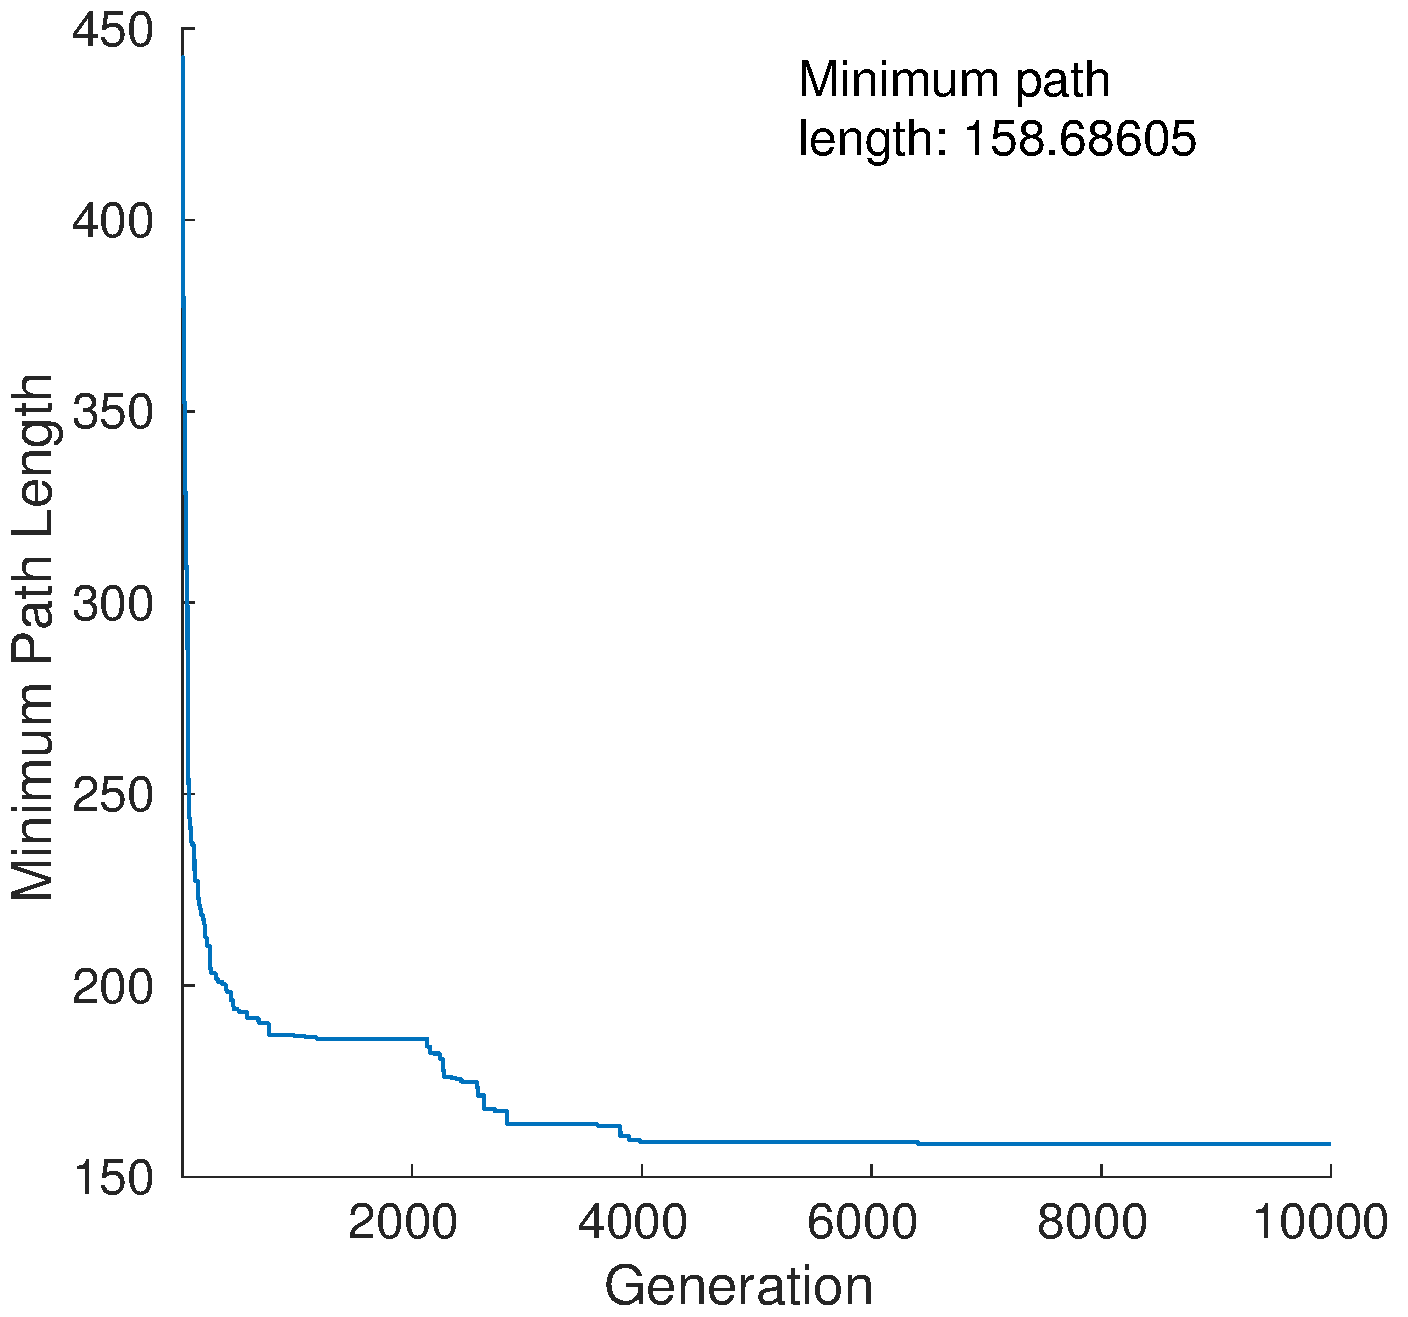
\includegraphics[width=\textwidth]{Figures/2b_minpathLength}
	\caption{}
	\label{subfig:2b_minPathLength}
\end{subfigure} %
\hfill %
\begin{subfigure}{0.45\textwidth}
	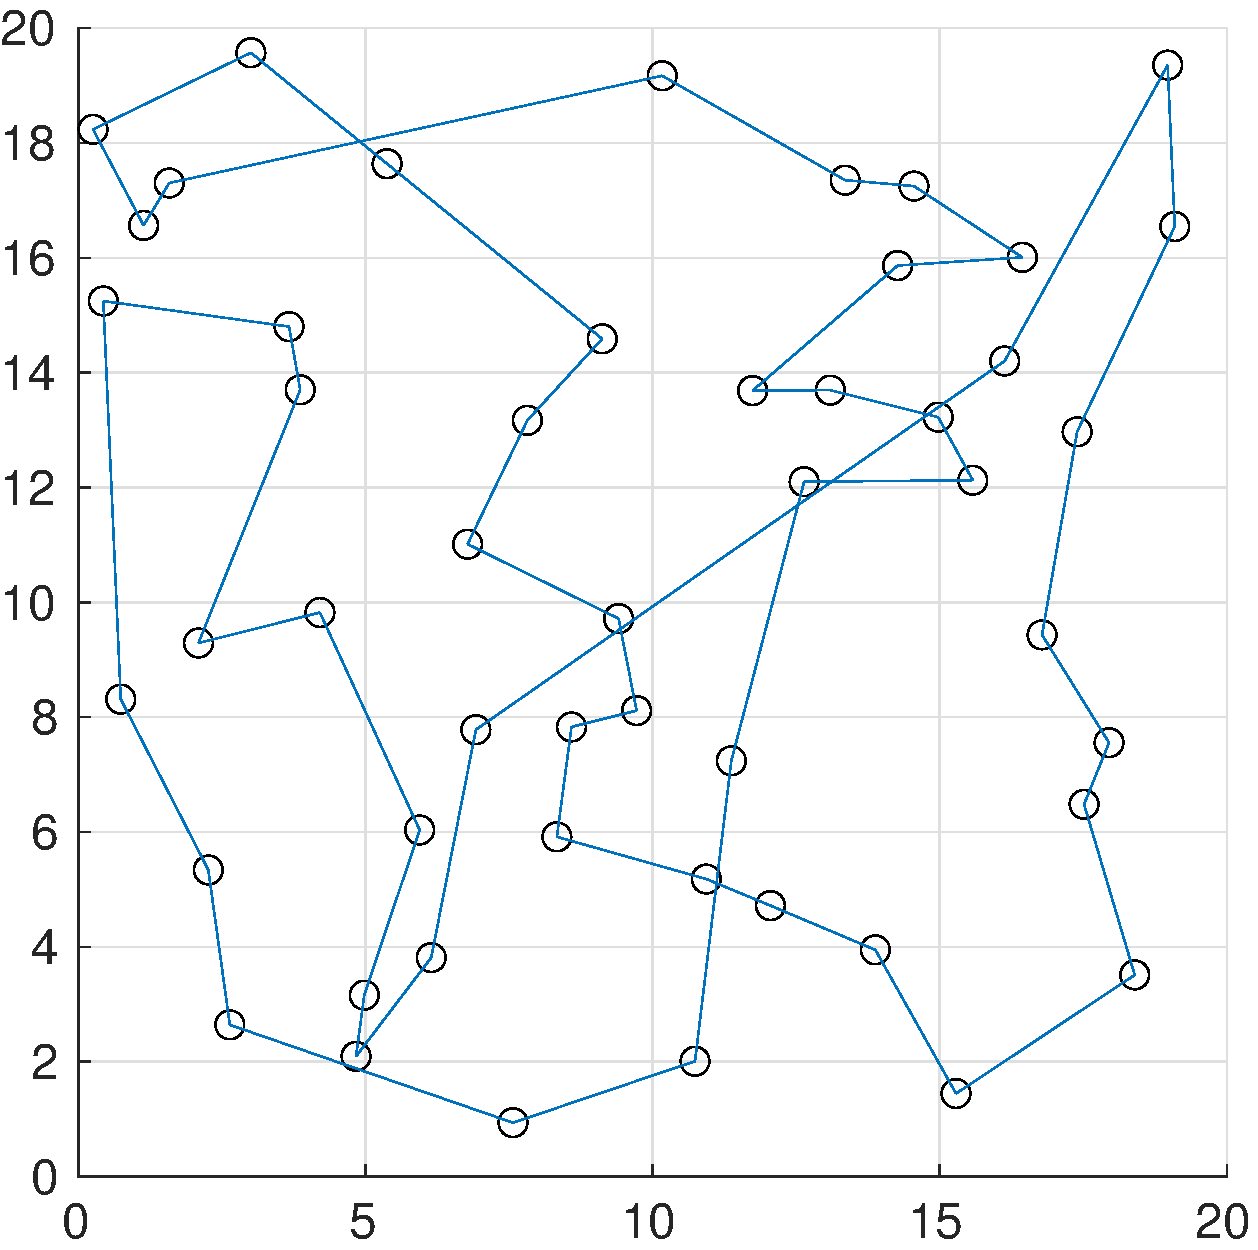
\includegraphics[width=\textwidth]{Figures/2b_pathPlot}
	\caption{}
	\label{subfig:2b_pathPlot}
\end{subfigure} %
\caption{Results of \texttt{GA21b} for TSP with random initial population. Left panel: minimum path length vs. generations. Right panel: best path found (length $\simeq$ 158.69).}
\label{fig:1b}
\end{figure}

\subsection*{2.1(c)}

An Ant System (AS) algorithm was implemented by completing the provided \textsc{matlab} script \texttt{AntSystem.m} and then applied to the same TSP as above. 

After experimenting with the parameters, it was found that using a larger number of ants than $N$ (number of cities) could help avoiding premature convergence, as more pheromone is deposited in each iteration. Path in Figure~\ref{fig:1c}, of length 122.44, was obtained by running the AS algorithm with 100 ants and parameters $\alpha = 2, \ \beta = 1, \ \rho = 0.5$, after 107 iterations. The AS algorithm was thus able to find a better solution than the GA, in a fraction of the time. The chromosome corresponding to this path is saved as a vector in file \texttt{bestPath.m} (in main folder \texttt{2.1}), which can be run as a script and loads the vector \texttt{bestPath} in the workspace.

\begin{figure}[htbp]
\centering
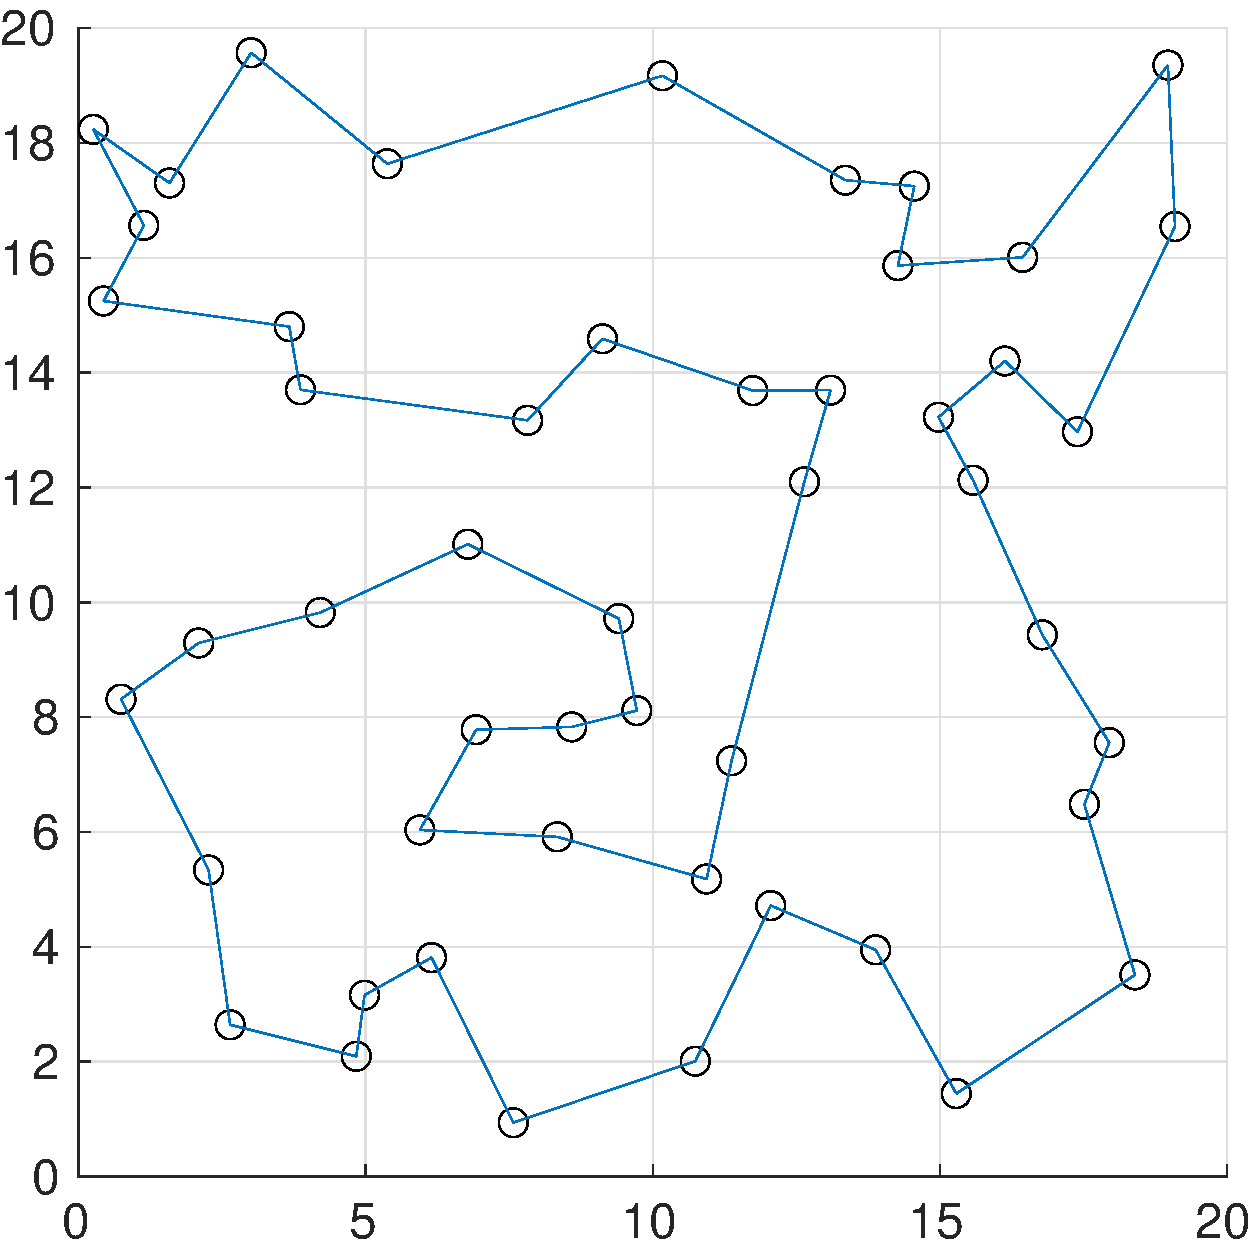
\includegraphics[width=0.45\textwidth]{Figures/2c_pathPlot}
\caption{Best path found with Ant System algorithm. Length $\simeq$ 122.44.}
\label{fig:1c}
\end{figure}

\subsection*{2.1(d)}
To allow a more fair comparison between GA and AS, the initialisation of the GA population was modified, so that starting path are nearest-neighbour paths (generated by starting from a random city) with a few random swap mutations (see function \texttt{InitializePopulation21d}).

Figure~\ref{fig:1c} shows the result of a long run (10000 generations) of the GA with 100 individuals and the same parameters as in 2.1(b), starting from a population of nearest-neighbour paths with 3 swap mutations each.
The length of the best path found by the GA in this case was $130.76$, so this solution is much better the one in 2.1(b), as expected, but not quite good as the solution found by using AS in 2.1(c).

\begin{figure}[htbp]
\centering
\begin{subfigure}{0.475\textwidth}
	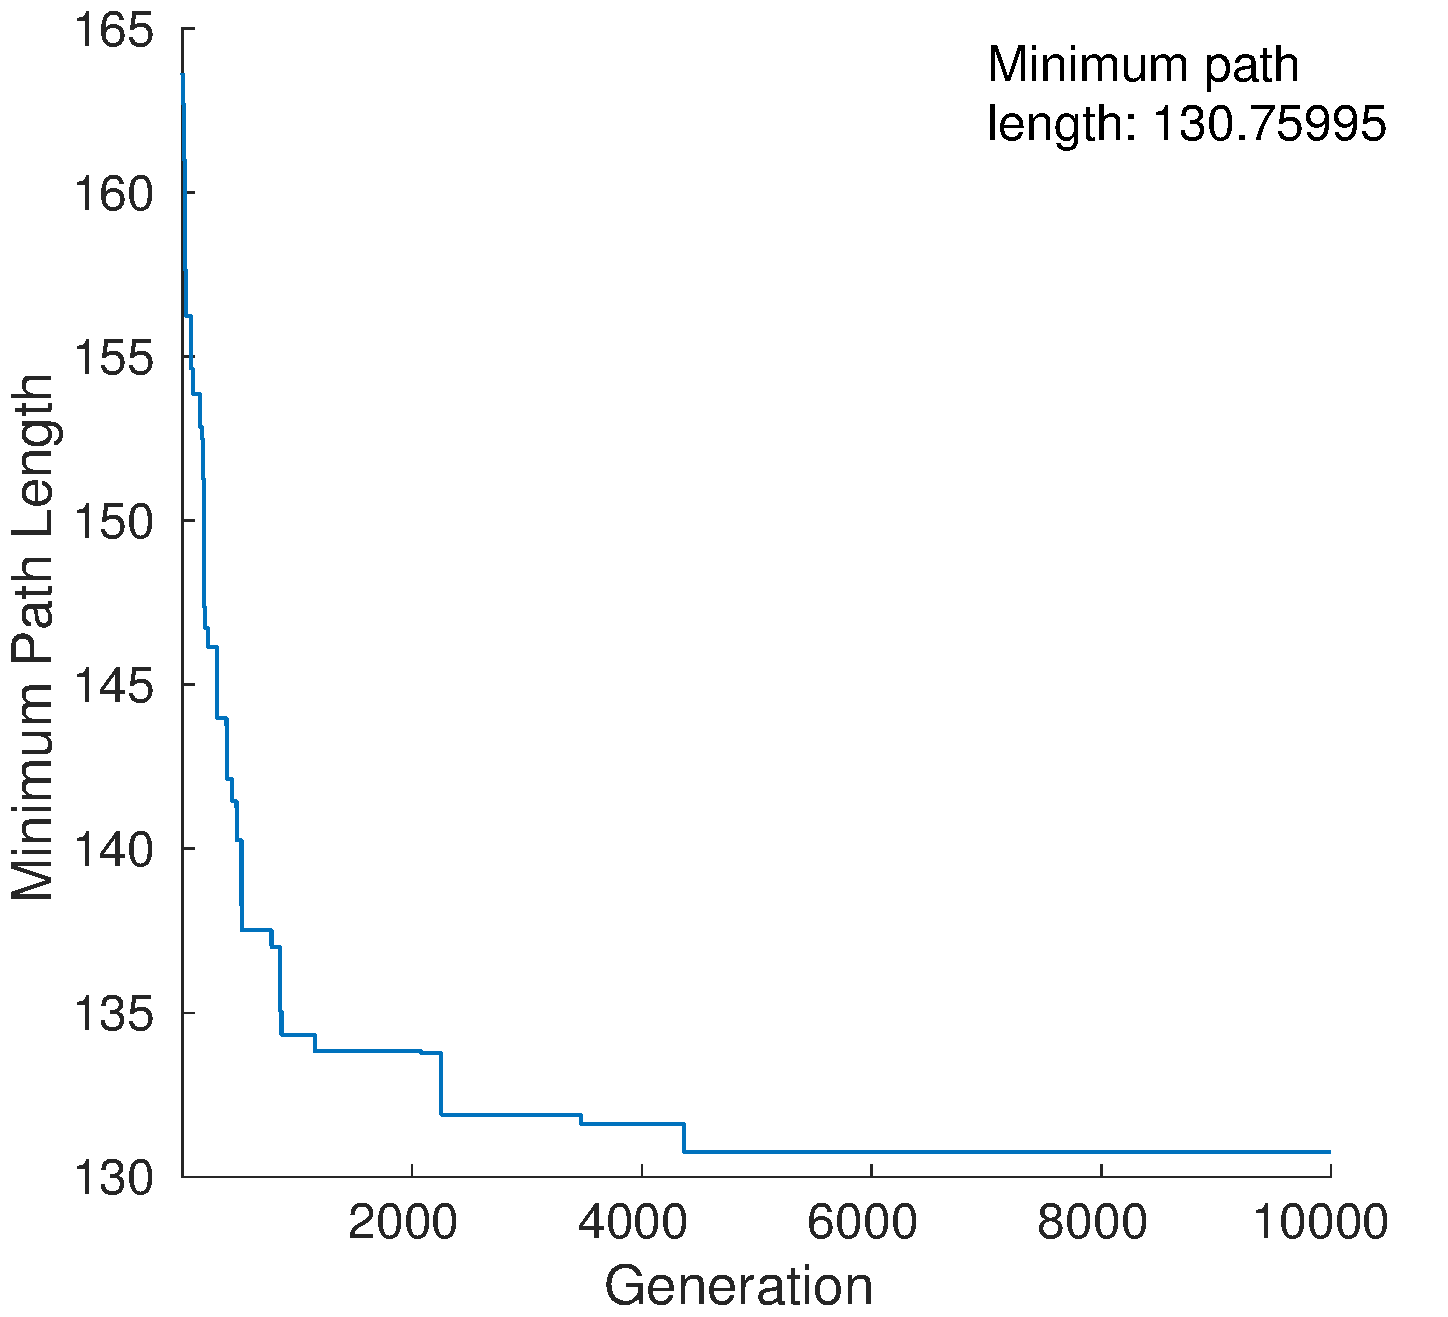
\includegraphics[width=\textwidth]{Figures/2d_minpathLength}
	\caption{}
	\label{subfig:2d_minPathLength}
\end{subfigure} %
\hfill %
\begin{subfigure}{0.475\textwidth}
	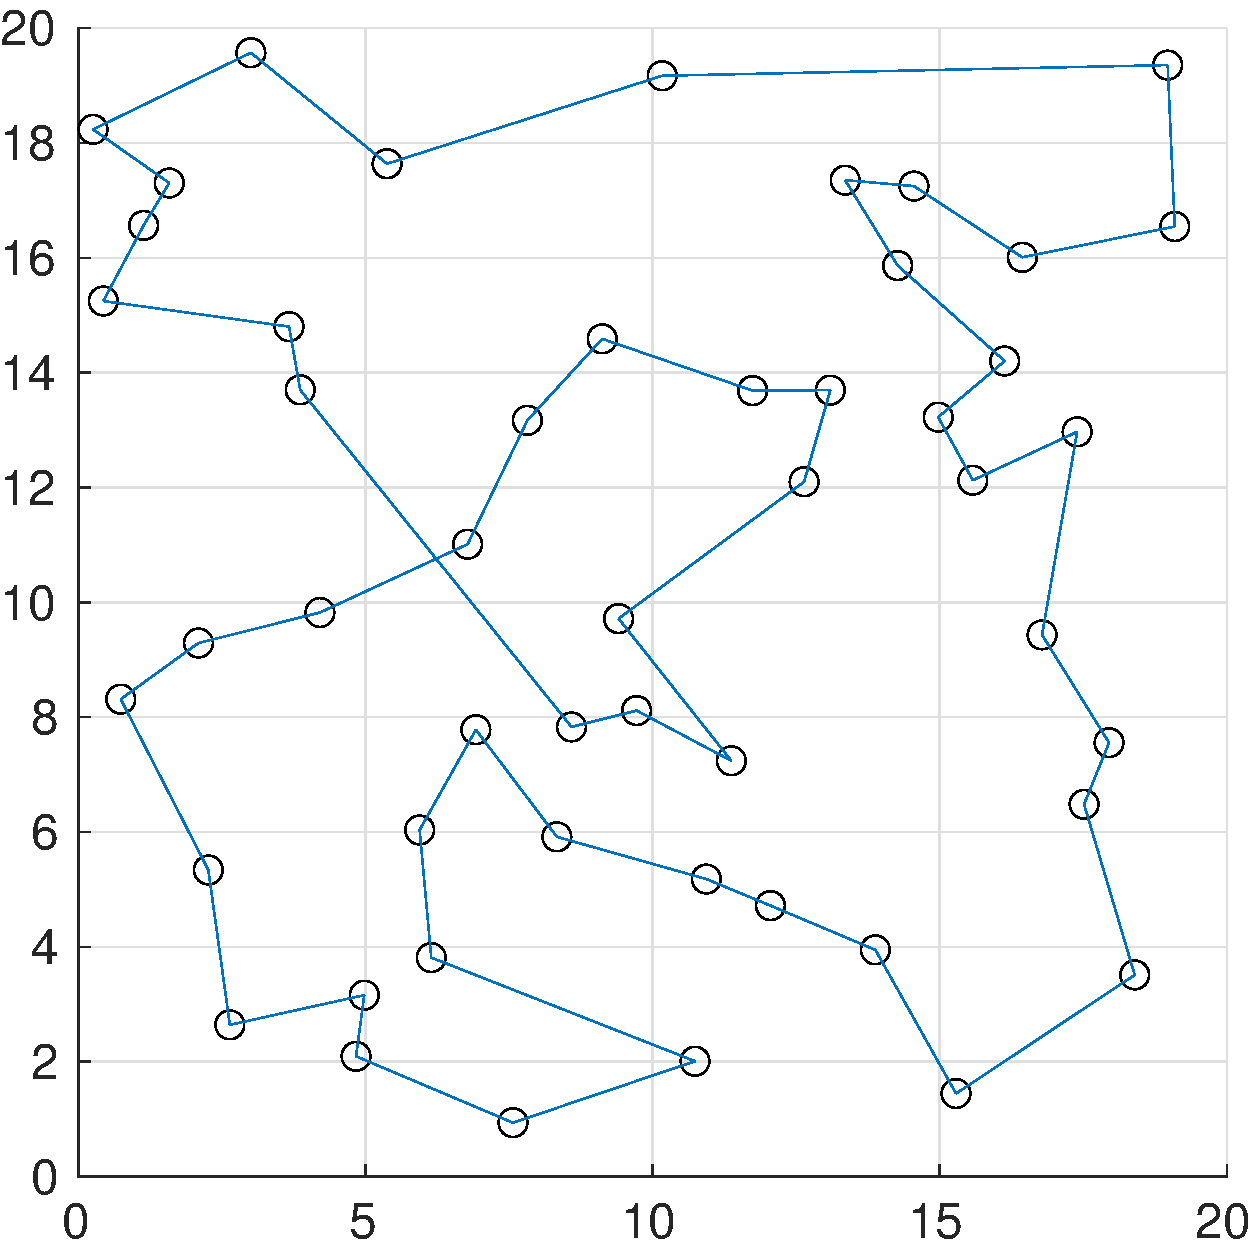
\includegraphics[width=\textwidth]{Figures/2d_pathPlot}
	\caption{}
	\label{subfig:2d_pathPlot}
\end{subfigure} %
\caption{Results of \texttt{GA21d} for TSP with initial population of nearest-neighbour paths with 3 swap mutations. Left panel: minimum path length vs. generations. Right panel: best path found (length $\simeq$ 130.76).}
\label{fig:1d}
\end{figure}

\section*{Problem 2.2 - Particle swarm optimisation}

\subsection*{2.2(a)}
\textsc{matlab} script \texttt{PSO22a} in folder \texttt{2.2/2.2a} contains an implementation of a standard PSO algorithm for function minimisation, with inertia weights and no craziness operator.

The algorithm was used to find the minimum of the function
\[
f(x, y) = 1 + (−13 + x − y^3 + 5y^2 − 2y)^2 + (−29 + x + y^3 	+ y^2 − 14y)^2 \ ,
\]
with $x$ and $y$ real values in $[-10, 10]$. 

After a few runs to explore the (rather small) parameter space, the settings in Table~\ref{tab:2a} were used to find the minimum
\[
(x^*,y^*)^T = (5.00, 4.00)^T \ , \qquad \mbox{with} \qquad f(x^*,y^*) = 1 \ .
\]

\begin{table}[hbtp]
\centering
\begin{tabular}{cccccccccc}
\toprule
Swarm & Number of &  &  &  &  & Maximum & Starting & Inertia weight & inertia weight \\
size & iterations & $ \alpha$ & $ \delta t$ & $ c_1$ & $ c_2$ & speed & inertia weight & decrease rate & inertia weight \\
\midrule
20 & 1000 & 1 & 1 & 2 & 2 & $ 20 \ (\alpha / \delta t) $ & 1.4 & 0.99 & 0.3 \\
\bottomrule
\end{tabular}
\caption{PSO settings and parameters used in \texttt{PSO22a}.}
\label{tab:2a}
\end{table}

\subsection*{2.2(b)}
The PSO was then modified to handle integer programming (see script \texttt{PSO22b} in folder \texttt{2.2/2.2b}). That is, when the objective function is evaluated, particle positions are temporarily rounded to the nearest integer values, whereas floating point values are using in all other stages of the computation.

The script was then used to find the minimum of the function
\[
f(\bm{x}) = -(15 \ 27 \ 36 \ 18 \ 12) \ \bm{x} + \bm{x}^T \ \begin{pmatrix}
35 & -20 & -10 & 32 & -10 \\
-20 &  40 & -6 & -31 & 32 \\
-10 & -6 & 11 & -6 & -10 \\
32 & -31 & -6 & 38 & -20 \\
-10 & 32 & -10 & -20 & 31 \\
\end{pmatrix} \ \bm{x} \ ,
\]
where $ \bm{x} = (x_1 , x_2 , x_3 , x_4 , x_5 )^T$, and $x_i \in \lbrace −30, −29, \ldots , 29, 30 \rbrace \in \mathbf{Z}$.

Using parameters in Table~\ref{tab:2b}, two minima (claimed to be global) were found:
\[
\bm{x^{*}}_{(1)} = (0, 11, 22, 16, 6)^T \ , \quad \mbox{and} \quad \bm{x^{*}}_{(2)} = (0, 12, 23, 17, 6)^T \ , \qquad \mbox{both with} \ f(\bm{x^*}_{(i)}) = -737 \ .
\]

\begin{table}[hbtp]
\centering
\begin{tabular}{cccccccccc}
\toprule
Swarm & Number of &  &  &  &  & Maximum & Starting & Inertia weight & inertia weight \\
size & iterations & $ \alpha$ & $ \delta t$ & $ c_1$ & $ c_2$ & speed & inertia weight & decrease rate & inertia weight \\
\midrule
50 & 2000 & 1 & 1 & 2 & 2 & $ 20 \ (\alpha / \delta t) $ & 1.4 & 0.99 & 0.3 \\
\bottomrule
\end{tabular}
\caption{PSO settings and parameters used in \texttt{PSO22b} (integer programming).}
\label{tab:2b}
\end{table}

\section*{Problem 2.3 - Optimisation of braking systems}





\end{document}

